\chapter{Methods}
\label{chapter:methods}

A properly planned project requires the analysis of multiple methods and strategies that can be applied during its design. 
Therefore, this chapter displays, focusing on the multiple aspects of the entire project, the different techniques, encountered revising the broad literature accessible in this field, and the decisions that brought to the actual development of the algorithm, which will be thoroughly described in the Chapter~\ref{chapter:implementation}.\\
In this chapter, an extensive outline of the work made is not produced, though. 
Instead, the following sections focus on a concise, yet exhaustive, tracing of the methods available for a correct dense disparity estimation and for image data processing.
Concurrently, the choices made for the specific aspect of the algorithm are defined and explained.

\section{Standard disparity estimation methods}
\label{section:std-methods}

An extensive and broad analysis of the standard and the deep learning methods for dense disparity estimation has already been presented in Chapter~\ref{chapter:background}, where the review of the literature related to this Master's thesis project has been carried out.
Nevertheless, these sections focus on a different aspect of that analysis, which is correlated to the algorithms that turned out to be the most relevant for this work and to the features of some of the current machine learning based techniques, which appear to be applicable to this project.\\
Considering the standard algorithms for recovering a dense depth image from a stereo pair, the initial approach on which it was decided to focus on for the designing of the project refers to the Semi-Global Matching (SGM) stereo method developed by Hirschm\"{u}ller~\cite{Hirschmuller2008}.
The decision of starting to concentrate on that evaluation of the stereo matching problem was mainly driven by the recent approaches designed for dense disparity estimation.
As a matter of fact, most of the algorithms created in the last decade are based on the Hirschm\"{u}ller idea or, at least, they make reference to several aspects of the functions outlined in~\cite{Hirschmuller2008}.
This fact is clearly comprehensible considering that the SGM method was classified as the best algorithm at the time of its publication and it is currently one of the top-ranked algorithm in terms of sub-pixel accuracy and computational time.
Hence, taking into account the benchmark data based on two of the most employed dataset, i.e. Middlebury~\cite{Scharstein2014} and KITTI~\cite{geiger2013vision} datasets, and after an initial general review of the literature publish in this field, it results that the top-performing algorithms use key features of the SGM in their main pipeline. 
Moreover, it is worth to point out that the majority of the most accurate real time deep learning based algorithm tends to adopt the main functions of the SGM model, exploiting neural networks to ensure real time evaluations of the disparities.
Therefore, it was initially though that a reasonable option for the development of an algorithm, which would work in real time providing accurate outcomes, would focus the attention of the Hirschm\"{u}ller method.\\
As already introduced in Section~\ref{section:stereo-methods}, the SGM method combines the idea of the standard local based algorithms, where the main cost calculations are made over limited size windows, and global algorithm, for which the best pixel disparity estimation is based on a global energy function. 
Thus, mainly because of its hierarchical cost calculation, SGM method outperformed the top-ranked algorithm over the dataset~\cite{scharstein2003high}, proving real-time performance over those images. 
However, with the current dataset, such as Middlebury 2014~\cite{Scharstein2014}, KITTI 2012~\cite{geiger2013vision} and KITTI 2015~\cite{menze2015object}, the standard SGM algorithm provide optimal results in terms of accuracy but it tends to slightly suffer if computational time is considered.
For this reason, the most recent real time methods for dense disparity estimation establish the cost computation part of their pipeline over the SGM idea, although, they exploit hardware efficiency or even neural network structures to reach extremely fast computations.\\
Thus, considering this project, it was decided to initially build up the main pipeline on the SGM method structure and employ the stereo device designed by the company to reach real time performance, without loosing in accuracy. 
Furthermore, as previously anticipated, an upstream choice was made. 
As a matter of fact, the current top-performing algorithms strongly depend on convolutional and deep neural network to achieve fast computations.
Contrarily to that, we decided to based the skeleton of our method on the data available through the stereo system to reach a real time implementation, similarly to what done in~\cite{Keselman2017}.
In this manner, all the problem related to the shifting between synthetic and real environment, faced by deep learning algorithms, would be avoided. \\
The first outline of the algorithm was, hence, partially based on the Semi-Global Matching method~\cite{Hirschmuller2008}. 
In order to analyse the suitability of the implementation, absolute computational time performances were not initially taken into account. 
At first it was chosen to focus on the relative efficiency that would be estimated among the different methods used in the principal pipeline.\\
As aforementioned in Chapter~\ref{chapter:environment}, these preliminary evaluations has been developed in MATLAB. 
In that phase an implementation sufficiently similar to the standard SGM method was designed. 
Thus, the focus was centred on the different types of algorithms used for matching the corresponding pixels and, then, on the part of the pipeline related to the matching and the aggregation costs, as precisely defined by Scharstein and Szeliski in~\cite{Scharstein2001}.
The employment of this working strategy was due to the following motivations. 
First of all, the predominant research aim of this project, whose purpose would only later shifts in more a market based perspective, then the need of testing the effective performance in accuracy of pure SGM based method and the requirement of analysing the relative efficiency between that algorithm and our method, whose pipeline would be based on the information acquired from the company stereo device. \\
A fundamental part of this initial testing phase was the focus on the matching cost evaluation, therefore, multiple matching cost algorithm has been tested in order to find the most efficient one mainly in terms of accuracy. 
Therefore, basing on the work done in~\cite{Hirschmuller2007}, \cite{Patil2013} and \cite{Ko2017}, and making reference to the algorithm used for computing visual correspondence described in~\cite{Zabih1994} and \cite{Demetz2013}, the performance of different matching cost algorithms has been analysed.

\subsection{Census transform}
\label{subsection:census-transform}

\begin{figure}[t]
	\begin{center}
	{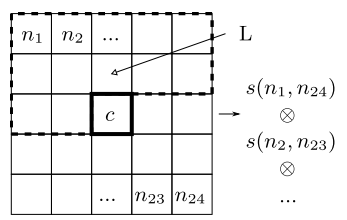
\includegraphics[width=.8\textwidth, height= 5cm, keepaspectratio]{images/center-symmetric-census.png}}
\caption{Center-Symmetric Census transform schema for a $5 \times 5$ image region. Credits to~\cite{Spangenberg2013}}
\label{fig:center-symmetric-census-schema}
	\end{center}
\end{figure}

A crucial phase of the SGM algorithm stands in the matching cost computation.
As briefly explained in Chapter~\ref{chapter:background}, this cost is evaluated by computing the difference in the value of intensity among corresponding pixels.
Therefore, especially when dealing with unexpected luminance variation inside the analysed scene, it comes out that non-parametric local transforms are optimal as the support for that correlation \cite{Zabih1994}.
As a matter of fact, these kind of measurements do not rely on the actual intensity values of the pixels, but on the relative local intensities instead.
Therefore, using this kind of models, a considerable number of outliers can be tolerated and improved results are visible especially along object boundaries.\\
Among the commonly used and best performing non-parametric local transforms, Census and Rank transform are described.
Moreover, couple of different implementations of those two classes of transform are introduced.\\
It is widely known in computer vision field that correspondence problem is crucial in depth estimation, when starting from stereo pairs.
Correspondence can be, thus, defined by transforming the images with a specific method and then establishing correlations.
In that, the key factor is the transformation, which must tolerate unexpected variation in intensity, for example due to unwanted light source, and in general changes in image bias and gain.\\
Therefore, non-parametric area-based transform rely on local ordering of intensities and not on the actual intensity values.
If an image is considered, and defining as $p$ a random pixel, its intensity becomes $I(p)$. 
Then, let $N_d(p)$ be the set of pixel in a certain square neighborhood of size $d$, where $p$ is the central pixel. 
Hence, the binary function $\beta(p, p')$ takes value 1 if $I(p') < I(p)$, 0 otherwise.
A non-parametric local transform only rely on the set of pixels in the specific neighborhood.
Therefore, the Census transform, $C_{\tau}(p)$ maps the image subregion surrounding $p$ to an array of bits representing the set of local pixels whose intensity is less or equal than that of $p$. 
Mathematically, the Census transform can be formulated as:
\begin{equation}
	\label{eqn:census-transform}
	C_{\tau}(p) = \bigotimes_{[i, j] \in D} \beta(p, p +[i, j])
\end{equation}
where, $N(p) = p \oplus D$, with $\oplus$ is the Minkowski sum and $D$ the set of displacements, and denoting with $\otimes$ the concatenation. 
After the Census transform has been applied, the actual comparison among corresponding pixels in done by computing their \textit{Hamming} distance.\\ 
Higher accuracy in corresponding pixel matching can be achieved using an extension of the Census transform, defined as Center-Symmetric Census transform~\cite{Spangenberg2013}.
Therefore, if a square image subregion is taken into account, which has dimensions $n \times m$, we already know from equation~\ref{eqn:census-transform} that $s(p, p') = 0, if p \leq p', 1$ otherwise, where now $s( )$ is the sign function.
Precisely, in this notation the Census transform can be thus defined as:
\begin{equation}
	\label{eqn:census-transf-2}
	CT_{m,n}(x, y) = \bigotimes_{i = -n'}^{n'} \bigotimes_{j = -m'}^{m'} s(I(x, y), I(x + i), y + j)
\end{equation}
where $n' = [n/2]$, and $m' = [m/2]$.
Hence, as shown in Figure~\ref{fig:center-symmetric-census-schema}, the Center-Symmetric Census transform can be mathematically defined as:
\begin{equation}
	\label{eqn:center-symmetric-census}
	CS-CT_{m,n}(x, y) = \bigotimes_{(i, j) \in L} s(I(x - i, y - j), I(x + i, y + j))
\end{equation}
where $L = L_1 \cup L_2$, $L_1 = R_{-n',0} \times R_{-m',0} \setminus {(0, 0)}$, $L_2 = R_{1,n'} \times R_{-m',1}$ and $R_{a, b} = {x \in \mathbb{Z} \vert a \leq x \leq b}$.
Because, only Center-Symmetric pairs of pixels are compared, the formulation in equation~\ref{eqn:center-symmetric-census} needs less bits than the one in~\ref{eqn:census-transf-2} to describe the same patch. 
As aforementioned, the actual matching cost is then computed using the Hamming distance between corresponding pixels. 

\subsection{Rank Transform}
\label{subsection:rank-transform}

\begin{figure}[t]
	\centering
	\subfigure[Grayscale pixel intensity values]{
 		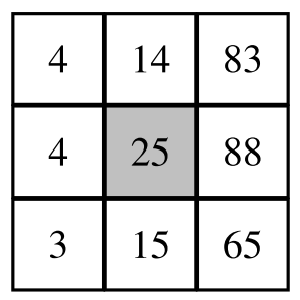
\includegraphics[width=0.3\textwidth, height= 5cm, keepaspectratio]{images/patch-rank-example.png}
}
	\subfigure[Rank transform ]{
 		 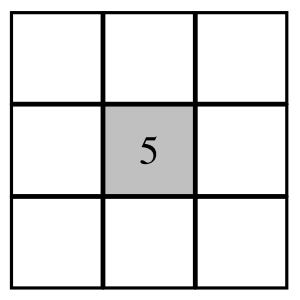
\includegraphics[width=0.3\textwidth, height= 5cm, keepaspectratio]{images/rank-signature.png}
}
\subfigure[Complete Rank transform]{
 		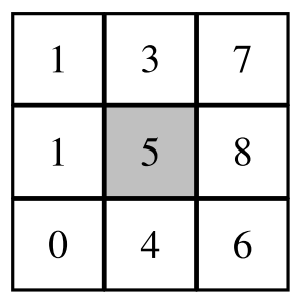
\includegraphics[width=0.3\textwidth, height= 5cm, keepaspectratio]{images/complete-rank-signature.png}
}
\caption{Example patch with grayscale pixel intensity values. Credits to~\cite{Demetz2013}}
\label{fig:rank-example}
\end{figure}

Another patch-based pixel descriptor is the Rank transform.
As the Census, it is morphologically invariant.
Therefore, it is not sensitive to any monotonically increasing of the grayscale intensity values. \\
The definition of this measure is, actually, quite simple.
The pixels in the specific patch considered are ordered basing on the ranking of all grayscale values in that area. 
Then, the reference pixel \textit{Rank encoding} is determined by counting the number of neighboring pixels with a gray intensity value smaller than the considered pixel, that is, basically, its position in the intensity ranking of the patch.
Figure~\ref{fig:rank-example} shows a $3 \times 3$ example patch where the central pixel, i.e. the reference one, is map to its scalar rank encode. 
This patch-based descriptor, as the Census transform, was introduced by Zabih and Woodfill~\cite{Zabih1994} and, defining an image pixel with $p$ and its neighborhood with $N(p)$, it can be mathematically expressed by the following equality:

\begin{equation}
	\label{eqn:rank-transform}
	R_{\tau}(p) = \Vert {p' \in N(p) \vert I(p') < I(p)} \Vert	
\end{equation}

Looking at the mathematics of the Census and the Rank transforms, it is evident that the former encodes more information. \\
In addition to the two presented non-parametric local transforms, there is another area based descriptor that need to be mentioned.\\
The Complete Rank transform can be thought as an improvement of the Rank transform.
It was more recently presented by Demetz et al.~\cite{Demetz2013}, with the goal of keep a higher amount of information with respect to its standard version.
Actually, it works in the following manner.
At first the normal Rank transform is applied to all the elements of the patch. 
Then, these ranks are concatenated, as it is done for the Census, so that the Complete Rank descriptor is generated.  
As visible in Figure~\ref{fig:rank-example}, pixels with the same intensity take the same rank value. 
Therefore, the encoding for the patch displayed in the image is:
\begin{equation}
	\label{eqn:complete-rank-encoding}
	\mathbf{enc}_{CRT} = (1, 3, 7, 1, 5, 8, 0, 4, 6)^\top
\end{equation}

\subsection{Conventional intensity based methods}
\label{subsection:conventional-methods}

Describe sum of absolute difference, sum of squared difference.
\section{Deep-learning based methods}
\label{section:deep-learning-method}

As introduced in section~\ref{subsection:deep-learn-meth} the deep learning method approach for stereo matching was not chosen as the base strategy for the development of this project for different reasons, which have already been explained in Chapter~\ref{chapter:background}.\\
However, the structure of a deep learning based project was extremely useful in the definition of the approach used for the designing of our work.
Fundamental is the novel stereo matching method developed by Poggi et al.~\cite{Poggi2019}, who exploited a small quantity of sparse initial depth data to enhance the overall stereo matching problem.
In their paper, they presented \textbf{\textit{Guided Stereo Matching}}, an innovative stereo algorithm, which uses a sparse set of accurate depth measurement obtained from reliable hardware system, e.g. a LiDAR, with the aim of improving the general performance of a standard depth estimation algorithm.\\
Therefore, considering the structure of our system, the strategy used in \cite{Poggi2019} appears to have valuable insights, which would be exploited in the definition of our own work.
Actually, they proposed to use sparsify yet reliable depth measurements for the following tasks: improve the general accuracy of the neural network designed for achieving the depth estimations, reduce the domain shift, i.e. the drops in accuracy that deep learning based methods face when dealing with data from a new environment, and the potential improvement of the result when training the network starting from that sparse set of inputs.\\
Similarly to that approach, in this project, we decide to base our overall estimations on the knowledge of the sparse group of 3D measurements coming from the LaDiMo stereo device.
However, differently from them, the algorithm described in this thesis uses standard methods in the stereo matching pipeline, which appear to work better for multiple types of environments. \\
Thus, taking into account the results provided in~\cite{Poggi2019}, where the authors demonstrate how their strategy outperforms the current state-of-the-art stereo matching methods, we assumed that a reasonable approach to apply would exploit the initial cues coming from the laser grid of points in order to improve the performance of the main algorithm. 
As a matter of fact, in their paper, Poggi et al.~\cite{Poggi2019} assert that the initial set of estimations can be obtained with whatever device that can give sparse data.\\
Consequently, during the initial stages of the development some tests have been performed designing a simulated point grid, in order to have a clear outcome of the reliability of this strategy.
Hence, employing the Middlebury 2014 dataset, the initial set of clues was designed taking the sparse depth information from the ground truth images available. 
Obviously, the depth measurements coming from the dataset can be considered highly accurate, differently from the data from the LaDiMo device, which would most likely be affected by some sort of noise, mainly Gaussian. 
Nevertheless, it is actually extremely useful to perform these tests in order to figure out since the first phases of the project, the qualitative performance of the adopted strategy.
The details of the conducted tests are widely described in Chapter~\ref{chapter:implementation}, where some of the temporary results obtained are also proposed.

\section{Pure derivative based data estimation algorithm}
\label{section:deriv-based-algorithm}

\begin{figure}[t]
	\begin{center}
		{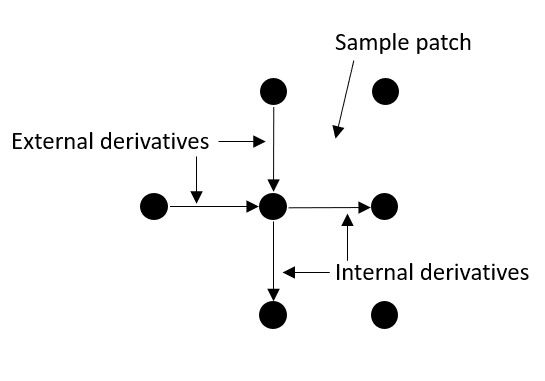
\includegraphics[width=.8\textwidth, height= 5cm, keepaspectratio]{images/sample-patch-derivative.png}}
\caption{Example of a 4-neighbors image patch where the internal and external derivatives related to one of the patch corners are highlighted}
\label{fig:example-patch-derivative}
	\end{center}
\end{figure}

As previously introduced, two different algorithm structures have been implemented and compared in this project, in addition to the standard Semi-Global Block Matching (SGBM) algorithm available in the OpenCV library, whose result was used as a baseline for carrying out an appropriate comparison with the novel implementation designed. \\
Therefore, the first one of these methods is closely related to the standard SGM implementation, it exploits the initial knowledge of the sparse depth estimations, however, the core of the algorithm follows the Hirshm\"{u}ller algorithm \cite{Hirschmuller2008}. 
Differently, the other implementation designed is more strictly related to the initial sparse depth clues, and it is focused on those for the overall pipeline of the algorithm.
As it will be reported in Chapter~\ref{chapter:evaluation}, this latter approach will provide a faster yet, in general, equally accurate implementation.
Therefore, these two designed strategies will be deeply explained in Chapter~\ref{chapter:implementation}.
Beside that, it is worth to propose here a concise outline of both of them, in order to introduce their main features.\\
Regarding the last introduced method, it highly exploits the information coming from the input sparse clues.
Therefore, starting from that initial 3D point cloud and using a pair of stereo images of the considered scene, a dense point cloud is built by estimating the space positions of an high amount of scene points. 
The key of this algorithm actually stands on the way in which those estimations are carried out. 
Thus, considering the point grid given by the stereo device, the local derivatives among neighboring points are evaluated. 
These will be then used for two main scopes: identify if inside a specific subpatch of the point cloud there could be an edge, that is that points belonging to the same small cluster have indeed highly different values of depth, and for computing the denser point cloud by interpolating the 3D value of neighboring points and exploiting the values of the pre-calculated derivatives for making the interpolation faster.\\
It can be, hence, easily understood how core of this strategy stands on the local derivatives calculation. 
As a matter of fact, let us consider a square cluster of 4 neighboring points from the initial point cloud, it is possible to evaluate the \textit{internal} and the \textit{external} derivatives among these points.
Specifically, the former are referred to be identified by the vectors that points \textit{inside} the square patch. 
Instead, the external derivatives are said to be the ones evaluated using the other points, which are neighbors to the patch corners. 
Figure~\ref{fig:example-patch-derivative} shows the aforementioned point cloud patch and the calculated derivatives relative to a corner. 
Summarizing, the denser 3D point cloud is estimated by filling up each one of the subpatches that can be identified from the initial grid. 
In order to perform this, the estimations are carried out exploiting the derivative vectors, which are weighted by the distance from the new estimated point and each one of the window corners.
This detail, in fact, shows that four temporary estimations are done for each new point. 
In this way, the best estimation is actually chosen by projecting the evaluated 3D point to the image plane and calculating the matching cost between the corresponding pixels for each temporary estimation.
For the matching cost, as it will be more widely explained in Chapter~\ref{chapter:implementation}, different methods have been investigated.
However, the plain absolute difference appeared to be the best in terms of performance for that algorithm.
In fact, at the end of the whole computation, similar results have been found with different matching cost algorithms.
Hence, in that case, it is worth nothing to use most expensive methods, which will make the computations heavier giving only slightly better results.
Besides that, specific penalties have been added on top of the pure matching cost to enhance the distance from the respective window corner in terms of $x$ and $y$ coordinates.\\
Summing up the general outcome gained from this approach, it results to be a lightweight yet effective method.
As it will be presented in the Chapter~\ref{chapter:evaluation}, this algorithm provides 3D dense point clouds that can be considered sufficiently accurate for a general use employing a relatively low amount of resources.
Despite that, internal parameters of that method can be adjusted, depending on the user needs, in order to obtain outcomes with a different grade of accuracy. 
Evidently, this will affect the performance in terms of computational time and used resources, however, this is always considered for every specific environment. 

\section{SGM based data estimation algorithm}
\label{section:sgm-based-algorithm}

As aforementioned, the second method that has been designed is based on a more standard approach, closely related to the SGBM algorithm. 
Basically, it exploits the information coming from the input point grid to make the standard pipeline of the SGBM method faster, which could be extremely expensive when dealing with high density images.
Actually, the initial points information is employed to select the disparity levels on which the main algorithm is run. 
Simply speaking, the final implementation can be considered as a \textit{disparity-wise} Semi-Global Block Matching, where, usually, there are not continuous changing in the disparity levels, especially if edges are detected inside the specific image patch.\\
Taking into account the general performance of this approach, it runs slower than the previous strategy. 
Moreover, the final 3D point cloud shows an higher density, however, looking at the achieved results, the increase in accuracy obtained in this case seems not to be worth the observed rising in computations. \\
Therefore, at the reached stage of the project, it appears that a slightly decrease in accuracy can be considered reasonable for a quite high increase in computation speed. \\
However, every use case has to be widely analysed in order to choose the most profitable solution.
Additionally, it is necessary to point out that this project should be regarded as still in a researching phase. 
Multiple tests have been performed with both dataset, i.e. almost perfect, and real images. 
However, for a good analysis of the specific use case, it is necessary to run various tests on the specific working environment, and eventually, adjusting parameters or side sections of the main pipeline.\\
Beside that, a further discussion over those topics will be presented in Chapter~\ref{chapter:discussion}. 
Anyhow, it was considered helpful for a deeper understanding of the results, which will be presented in Chapter~\ref{chapter:evaluation}, to introduce also here some brief comments over the outlined algorithms.\\
Hereafter, a short overview on the pre and post-processing techniques employed in the whole project is presented. 
Further details will be described in the following chapter. 
Anyway, it is useful to introduce here the main techniques used and especially the differences in performance, which have been analysed, and also their scope in relation to the final accuracy of the algorithms.

\section{Pre-processing techniques}
\label{section:pre-process-tech}

In the first section of the algorithm pre-processing techniques have turned out to be, not indispensable, but useful for the accuracy of the final results.
The focus was especially centred on the noise removal. 
As a matter of fact, if a stereo pair is given, it is generally affected by Gaussian, i.e. random, noise, which can be due to multiple reasons, such as instability of environmental conditions, lightning, local temperature gradients that can affect the stereo system or errors in the setting of the stereo device. \\
Therefore, for those reasons and for the purpose of launching the algorithm having the input image as clearer as possible, especially in terms of pixels' intensity, blurring filters have been tested and analysed during the development of this first phase of the pipeline. 
Specifically, median and bilateral filters occur to be ideal for smoothing away noisy components in the frequency spectrum, keeping the performance of the whole algorithm reasonable. \\
The details of that analysis are left to Chapter~\ref{chapter:implementation}.
However, it is worth to indicate that, even if more computationally expensive, the median filter comes out as the preferred choice for image blurring when dealing with real stereo pairs.
As a matter of fact, when the images from the datasets have been tested, there was not any needs to apply some sort of pre-processing, being them already cleaned from noisy components. \\
Contrarily, talking about the real dataset and especially about the initial grid of points obtained from the LaDiMo stereo device, some pre-processing operations have been performed over those data too. 
The goal of this process was the requirement of starting the main computations basing on accurate and possibly complete data. 
Focusing on that, it actually happened that the input point cloud was, in general, not fully complete. 
Instead, some of the points had missing data.
This was probably due to occlusions, in fact most of the \textit{bad} points areas were located on edges or on regions affected by shadows. \\
Therefore, this problem was tackled in the following way.
First of all, all those input data have been analysed and, specifically, the percentage of completely missing values with respect to the total amount of points was calculated. 
This was performed to obtain an initial estimation of the percentage of errors present in the input data, thus to evaluate the degree of effort that it should be required to have a final accurate result.
Precisely, let us think about the case of having an extremely low amount of errors, e.g. the 1.5\% of the entire point cloud. 
Moreover, consider the condition in which these errors are sparsified.
In this case would be rather complicated to fill in those missing data.
Thus, it would be worth nothing to spend resources to improve the completeness of the input data, reaching an outcome that would be, most likely, only slightly more accurate and for which the whole algorithm would be way computationally heavier and more complicated. 
On the contrary, a feasible option can be the one of running multiple time a very lightweight algorithm, exploiting the most accurate new estimated points to improve the density of the successive 3D clouds.\\
For the actual purposes of this chapter it is unnecessary to present further details of this data processing, which would be more widely analysed in the following sections. \\
On the other hand, it is convenient to introduce here some features about the post-processing operations, which have been carried out in the last section of the algorithm.

\section{Post-processing techniques}
\label{section:post-process-tech}

Considering the results achieved with both the Middlebury 2014 dataset and the real environment images an additional blurring process has been run over the final data. 
Differently from the the smoothing operations employed in the first part of the depth estimation method, in this phase the morphological filters emerge to be the most appropriate trade-off between final result and computational resources. \\
Also during the designing of this area of the project several tests have been carried out in order to obtain an estimation of the most suitable post-processing technique to run over the final result.\\
Therefore, considering the disparity images achieved using the stereo pair from the \textit{perfect} Middlebury dataset, the application of an additional median filter seemed more appropriate.
However, for the outcome accessed using images taken with the LadiMo device, the use of morphological filters appear more convenient. 
Additionally, several of those have been tested. 
Opening, closing, erosion and dilation have been run over both the raw disparity result and over the raw denser 3D point cloud.
Moreover, in order to have a clear idea of the performance of the different kernels, even mixture of those morphology operations have been generated. \\
At the end, the application of an opening filter gave the most accurate result on the 3D point cloud. 
